\documentclass[10pt,a4paper]{article}

\usepackage{enumerate}
\usepackage[top=2in, bottom=1.5in, left=1in, right=1in]{geometry}
\usepackage{fancyhdr} 		% page header
\usepackage{listings} 		% present source code.
\usepackage{amsmath}
\usepackage{amssymb}
\usepackage{float}
\usepackage{graphicx}
\usepackage{epstopdf}
\usepackage{hyperref}
\usepackage{lipsum}			% just to generate text for the example
\usepackage{verbatim}
\usepackage{tikz}

\pagestyle{fancy} 
\fancyhf{}
\fancyhead[L]{CS 540-1}
\fancyhead[R]{Fall 2018}

\def\x{\mathbf{x}}
\def\y{\mathbf{y}}
\def\w{\mathbf{w}}
\def\p{\mathbf{p}}

\begin{document}

\begin{center}
{\bf \large CS 540-1: Introduction to Artificial Intelligence

Homework Assignment \# 4

\vspace{0.5cm}

Assigned:  Thursday, 9/27  

Due:  Thursday, 10/4 before class} 
\end{center}

\vspace{1cm}

\begin{center}
{\bf \Large Hand in your homework:}
\end{center}


This homework is a programming assignment. Please hand in the Java program
\texttt{RingTreblecross.java}, completing the code skeleton we have provided. You
are required to \textbf{use only built-in libraries} to complete this
assignment. You may define your own classes for this assignment. \textbf{Do not
  include any package statements} in your submission. Go to UW Canvas, choose
your CS540-1 course, choose Assignment, click on Homework 4: this is where you
submit your file.

\section*{Question 1: $(n,k)$-Ring Treblecross}
For this assignment, you will be implementing the minimax algorithm in order to
play the game of $(n,k)$-Ring Treblecross.\\

$(n,k)$-Ring Treblecross is a variant of tic-tac-toe with the following key differences:
\begin{enumerate}
\item It is played on a ring-shaped board with $n$ positions.
\item Both players place X pieces on the board.
\item The game is won when a player achieves $k$ OR MORE consecutive X pieces on the
  board. See below for an example of (12,3)-Ring Treblecross.
\end{enumerate}

\begin{figure}[h]
	\centering
	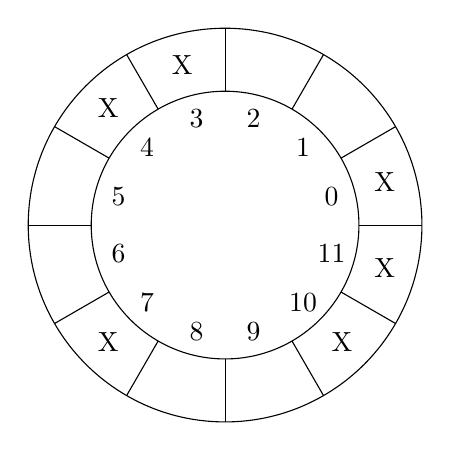
\begin{tikzpicture}
	\draw (0,0) circle (2.5cm);
	\draw (0,0) circle (1.7cm);
	\foreach \a in {0, 30,...,359}
	\draw (\a:1.7cm) -- (\a:2.5cm);
	\draw (15: 1.4) node {0};
	\draw (45: 1.4) node {1};
	\draw (75: 1.4) node {2};
	\draw (105: 1.4) node {3};
	\draw (135: 1.4) node {4};
	\draw (165: 1.4) node {5};
	\draw (195: 1.4) node {6};
	\draw (225: 1.4) node {7};
	\draw (255: 1.4) node {8};
	\draw (285: 1.4) node {9};
	\draw (315: 1.4) node {10};
	\draw (345: 1.4) node {11};
	\draw (315: 2.1) node {X};
	\draw (345: 2.1) node {X};
	\draw (15: 2.1) node {X};
	\draw (105: 2.1) node {X};
	\draw (135: 2.1) node {X};
	\draw (225: 2.1) node {X};
	\end{tikzpicture}
	\caption{A completed game of Ring Treblecross for $k = 3$.}
	\label{fig:fig1}
\end{figure}

In your implementation, both $n$, the size of the board, and $k$, the number of
contiguous pieces that need to be placed for the game to be won, will be
specified as command line parameters to your program.

Given a current state for the board where the next move is yours, your task is to
make the best next move. That is, you need to find the best possible placement
of X using a minimax search from the current state down to the leaves. Note
that the current state need not be an optimally-played configuration and can
have multiple pieces on the board.

The rules of the game are as follows:
\begin{enumerate}
\item The game is played by two players who alternate turns placing an X on the board at some unoccupied square. 
%\item The code is always the MAX player. The player who moves first (places the first X on the empty board) is considered the MAX player. The other player is the MIN player.  In the code , the code is actually hard coded to be a max player against human. 
\item A player wins by achieving $k$ OR MORE consecutive pieces on the board.
\end{enumerate}


\vspace{0.5cm}

\textbf{\Large Your mission, should you choose to accept it...}


\begin{enumerate}
\item To complete this assignment, it is sufficient to complete the code template
marked by ``TO DO'' in the provided source file.
\item  You are
free to define any helper methods you would like. However, you should not define
any additional member variables or class variables as they will likely only
increase the chances of unexpected bugs in your implementation.
\item In particular, you \textbf{must not} modify any other method bodies other than the 4 methods
we have marked in the source.
\end{enumerate}

\textbf{\Large Program Specification}

\begin{enumerate}
\item Command line arguments specify the following: the board size $n$, the
  parameter $k$ of contiguous pieces defining the least winning condition of the game,
  an operating flag which will determine the output of the program, and a variable-length list of integers defining the
  configuration of the board. For example:
\begin{verbatim}
java RingTreblecross 6 3 0 1 5
\end{verbatim}
  will begin a game on a board of size 6 where 3 contiguous pieces OR MORE are required
  to win the game. The operating flag \texttt{0} causes the program to execute
  an interactive game where you can play against your code.
  The first three arguments are required. The remaining (optional and variable length)
  arguments \texttt{1 5} specify the initial board configuration. As you can see
  positions \texttt{1} and \texttt{5} are occupied by X pieces. And you are
  prompted to input your next move.

\begin{verbatim}
Initial :  |   | X |   |   |   | X |
Choose Next Move:
\end{verbatim}
  
  Inputting \texttt{0} is a winning move here, and if you enter it, the program
  will terminate. Otherwise, the opponent will move and you will be prompted
  again for your move, until the game is over.

\item A state where MAX player wins is scored +1;  A state where MIN player wins is scored -1.

\item We require the code to return a list of successor from \texttt{getSuccessors} method in a specific order.
In particular, the successor must be sorted by the index of the ``filled-in'' square.
For example, the initial state
\begin{verbatim}
|   | X |   |   |   | X |
\end{verbatim}
should produce a list of successors in this order: 
\begin{verbatim}
0: | X | X |   |   |   | X |
1: |   | X | X |   |   | X |
2: |   | X |   | X |   | X |
3: |   | X |   |   | X | X | 
\end{verbatim}
This is because successor 0 filled in the empty square at index 0 in the initial state, successor 1 filled in the square at index 2, and so on.

\item It is possible that multiple successors of a state have the same score. For tie breaking, the \texttt{maxValueAndBestSuccessor} and \texttt{minValueAndBestSuccessor} methods should use the first successor with the best score from
getSuccessors method as the best successor. 

\item The following operating flags are defined:
\begin{enumerate}
  \item \texttt{0}: Play an interactive game against the algorithmic opponent beginning
    at the specified position.  Human moves first.
  The code template will call your code when it is your code's turn to move.
  See above for an example.
  
  \item \texttt{1}: Print all the successors of the board position specified on
    the command line as well as their game-theoretic score. 
    Your code is ALWAYS THE MAX PLAYER.
    For example,
    \texttt{java RingTreblecross 3 3 1}, on a correct implementation, should print
    the following output:
\begin{verbatim}
Min Node  | X |   |   |  Score:  1
Min Node  |   | X |   |  Score:  1
Min Node  |   |   | X |  Score:  1
\end{verbatim}
  \item \texttt{2}: Print a trace of an optimal sequence of moves beginning from
    the board position specified at the command line. For example, \texttt{java
      RingTreblecross 7 3 2}, on a correct implementation, should print the
    following output:
\begin{verbatim}
Max Node  |   |   |   |   |   |   |   |  Score: -1
Min Node  | X |   |   |   |   |   |   |  Score: -1
Max Node  | X |   |   | X |   |   |   |  Score: -1
Min Node  | X | X |   | X |   |   |   |  Score: -1
Max Node  | X | X | X | X |   |   |   |  Score: -1
\end{verbatim}
    \item \texttt{3}: Print the best successor of the board position specified
      on the command-line. For example, \texttt{java RingTreblecross 10 3 3 5}, on a
      correct implementation, should output:
\begin{verbatim}
Min Node  | X |   |   |   |   | X |   |   |   |   |  Score:  1
\end{verbatim}
\end{enumerate}

\item Note that all the code to parse the command line arguments has been
  written for you. We will not test your code on invalid inputs. Do not worry about
  input error-handling.

\item The board is represented in the provided code skeleton as of type
  \texttt{boolean[]}, an array of boolean values. Think of the squares of a
  board of length $n$ as indexed $0$ to $n-1$, reading from left to right. The
  $i$-th element in the boolean array represents the $i$-th squre of the board
  and contains the value \texttt{true} if the corresponding board position
  contains an X.
 
\end{enumerate}
\end{document}
